\documentclass{ctexart}
\usepackage{PhysicalChemistryNote}

\begin{document}\pagestyle{plain}
\Section{7D.3 酶促反应动力学}
\indent 迄今为止,我们还没有系统地讨论有催化剂参与时反应的动力学特征.%
尽管在前面,我们已经讨论了一类自催化反应,但大多数时候催化剂都是额外加入的,在总反应中不会被消耗的物质.\\
\indent 我们在本节要讨论的催化剂,\tbf{酶},就是一种高效专一的生物均相催化剂.关于酶的基本概念与特性,你可以查阅生物化学书.%
我们在这里主要关注酶催化的反应,即\tbf{酶促反应}的动力学特性.\vspace{4pt}\\
\Part{简单酶促反应与米氏方程}
\indent 最简单的酶催化反应的机理可由以下基元反应描述.
\begin{tightcenter}
    \ce{E + S <=>T[$k_1$][$k_{-1}$] ES ->T[$k_2$] E + P}
\end{tightcenter}
其中\ce{E}即参与催化的酶,\ce{S}为底物(即反应物),\ce{ES}为酶-底物复合中间体,\ce{P}为产物.%
我们现在来推导该反应的速率方程.
\begin{derivation}
    对中间体\ce{ES}做稳态近似可得
    \[\dfrac{\di\con{ES}}{\di t}=k_1\con{E}\con{S}-k_{-1}\con{ES}-k_2\con{ES}=0\]
    于是有
    \[\con{ES}=\dfrac{k_1\con{E}\con{S}}{k_{-1}+k_2}\]
    根据催化剂的物料守恒可得
    \[\con{E}+\con{ES}=\con{E}_0\]
    于是
    \[\con{E}=\dfrac{\con{E}_0}{1+\dfrac{k_1\con{S}}{k_{-1}+k_2}}\ \ \ \ \ 
    \con{ES}=\dfrac{k_1\con{E}_0\con{S}}{k_{-1}+k_2+k_1\con{S}}\]
    于是反应的速率即为
    \[\dfrac{\di\con{P}}{\di t}=k_2\con{ES}=\dfrac{k_1k_2\con{E}_0\con{S}}{k_{-1}+k_2+k_1\con{S}}\]
    为了简化上式,我们不妨定义$K_M=\dfrac{k_{-1}+k_2}{k_1}$,这样就有
    \[\con{ES}=\dfrac{\con{E}\con{S}}{K_M}\]
    同理,最后可以得出
    \[\dfrac{\di\con{P}}{\di t}=\dfrac{k_2\con{E}_0}{1+\dfrac{K_M}{\con{S}}}\]
    如果底物\ce{S}大大过量,那么就有$\dfrac{K_M}{\con{S}}\sim0$,于是
    \[\dfrac{\di\con{P}}{\di t}=\dfrac{k_2\con{E}_0}{1+\dfrac{K_M}{\con{S}}}\approx k_2\con{E}_0\]
    这就是酶的总浓度一定时反应的最大速率,记作$v_{\max}$.如此,速率方程亦可以写作
    \[v=\dfrac{v_{\max}}{1+\dfrac{K_M}{\con{S}}}\]
    
\end{derivation}
这就是Leonor Michaelis和Maud Menten提出的\tbf{米氏方程}.
\begin{theorem}[7D.3.1 米氏方程]
    对于符合
    \begin{tightcenter}
        \ce{E + S <=>T[$k_1$][$k_{-1}$] ES ->T[$k_2$] E + P}
    \end{tightcenter}
    机理的酶促反应,其速率方程为
    \[v=\dfrac{v_{\max}}{1+\dfrac{K_M}{\con{S}}}\]
    其中\tbf{米氏常数}$K_M=\dfrac{k_{-1}+k_2}{k_1}$.$v_{\max}=k_2\con{E}_0$,是该反应在酶的总浓度$\con{E}_0$一定时能达到的最大速率.
\end{theorem}
以下是$v$对$\con{S}$作图的结果.可以看出,当$\con{S}\ll K_M$时近似地有$v=\dfrac{v_{\max}}{K_M}\con{S}$,反应对\ce{S}为准一级.%
当$\con{S}\gg K_M$时,反应速率趋近于$v_{\max}$,反应对$\con{S}$为准零级.
\begin{tightcenter}
    \documentclass{standalone}
\usepackage{PhysicalChemistryNote}
\begin{document}
\begin{tikzpicture}
    \draw[->] (0,0)--(6,0) node[right]{$\con{S}$};
    \draw[->] (0,0)--(0,4.5) node[above]{$v$};
    \draw[domain=0.0001:6] plot[smooth](\x,{4/(1+0.5/\x)});
    \draw[dashed] (0,4)--(6,4);
    \fill (0,4) circle (1.5pt) node[left]{$v_{\max}$};
\end{tikzpicture}
\end{document}
\end{tightcenter}
\indent 反应速率常数$k_1,k_{-1},k_2$是较难直接获取的,但米氏方程为我们提供了线性回归测定它们的方式.%
将米氏方程变形可得
\[\dfrac{1}{v}=\dfrac{1}{v_{\max}}+\left(\dfrac{K_M}{v_{\max}}\right)\dfrac{1}{\con{S}}\]
可以看到,$\dfrac{1}{v}$与$\dfrac{1}{\con{S}}$成一次函数关系.测定\ce{S}在不同起始浓度$\con{S}_0$及其对应的速率$v_0$,%
就可以通过线性回归的方式求出斜率$\dfrac{K_M}{v_{\max}}$和截距\footnote{如无特别说明,截距一般指$y$轴截距.}$\dfrac{1}{v_{\max}}$.%
这种方式就是\tbf{Lineweaver-Burk作图法}\footnotemark\footnotetext{分别译作“莱恩威弗-伯克作图法”,“哈尼斯-伍尔夫作图法”和“伊迪-霍夫斯蒂作图法”.}.
\begin{theorem}[7D.3.2 Lineweaver-Burk作图法]
    在符合米氏方程的酶促反应中,反应速率的倒数$\dfrac1v$和底物浓度$\dfrac{1}{\con{S}}$成一次函数关系,根据实验数据作图就可以求得米氏常数$K_M$.%
    因此,这一方法也被称作\tbf{双倒数法}.
\end{theorem}
下面是由Lineweaver-Burk作图法给出\tbf{7D.3.1}的图像.
\begin{tightcenter}
    \documentclass{standalone}
\usepackage{PhysicalChemistryNote}
\begin{document}
\begin{tikzpicture}
    \draw[->] (-2.5,0)--(4,0) node[right]{$\dfrac{1}{\con{S}}$};
    \draw[->] (0,0)--(0,3.5) node[left]{$\dfrac{1}{v}$};
    \draw[dashed] (-2,0)--(1,1.5);
    \draw[-] (1,1.5)--(4,3);
    \fill (0,1) circle (1.5pt) node[above left]{\small{$\dfrac{1}{v_{\max}}$}};
    \fill (-2,0) circle (1.5pt) node[below]{\small{$-\dfrac{1}{K_M}$}};
    \node at (2,0.5) {\small{$\dfrac{1}{v}=\dfrac{1}{v_{\max}}+\left(\dfrac{K_M}{v_{\max}}\right)\dfrac{1}{\con{S}}$}};
\end{tikzpicture}
\end{document}
\end{tightcenter}
通过$x$轴截距和$y$轴截距就能计算出$v_{\max}$和$K_{M}$.%
不过,这一方法仍不能给出$k_1$和$k_{-1}$的具体值.%
我们需要更复杂的手段进行测量,这里就不再赘述.\\
\indent Lineweaver-Burk作图法仍然存在一些缺陷.只有当$\con{S}$相当小时,我们才能获取远离$y$轴的数据点.%
对于一般浓度的\ce{S},对应的数据大多靠近$y$轴,较为密集,在线性回归时容易引起误差.因此,可以对作图的直线表达式两端同乘$\con{S}$,即有
\[\dfrac{\con{S}}{v}=\dfrac{\con{S}}{v_{\max}}+\dfrac{K_{M}}{v_{\max}}\]
通过$\dfrac{\con{S}}{v}$对$\con{S}$作图,得到斜率为$\dfrac{1}{v_{\max}}$,截距为$\dfrac{K_M}{v_{\max}}$的直线.这就是\tbf{Hanes-Woolf作图法}\footnotemark[\arabic{footnote}].\\
\indent 当然,你还可以对\tbf{7D.3.1}变形得到
\[\dfrac{v}{\con{S}}=\dfrac{v_{\max}}{K_M}-\dfrac{v}{K_M}\]
通过$\dfrac{v}{\con{S}}$对$v$作图,得到斜率为$-\dfrac{1}{K_M}$,截距为$\dfrac{v_{\max}}{K_M}$的直线.这就是\tbf{Eadie-Hofstee作图法}\footnotemark[\arabic{footnote}].\vspace{4pt}\\
\Part{竞争性抑制剂和非竞争性抑制剂}
\indent 酶对反应体系是敏感的.一些物质可以与酶发生反应,进而降低其活性或使其完全失效.这就是\tbf{抑制剂}.
\begin{definition}[7D.3.3 抑制剂]
    \tbf{酶抑制剂}是一类特异性作用于或影响酶的活性中心或必需基团,导致酶活性下降或丧失,进而降低酶促反应速率的物质.
\end{definition}
按照抑制剂作用的机理不同,酶抑制剂可以简单地被分为如下两类.
\begin{definition}[7D.3.4 抑制剂的分类]
    \tbf{竞争性抑制剂}在结构上通常与底物相似.它和底物不能同时与酶结合,通常是由于它和底物对酶的同一活性位点都具有亲和力,故底物和抑制剂竞争结合该位点,从而使得反应减缓.\\
    \tbf{非竞争性抑制剂}通常与酶的非活性部位结合,改变酶的结构,从而降低酶的活性,但不影响酶与底物结合.\\
    \tbf{反竞争性抑制剂}仅与酶-底物复合物结合,导致其不能正常发生分解而生成产物.\\
    \tbf{复合抑制剂}可以与酶或酶-底物复合物结合,使得反应的速率减缓.\\
    以上四种抑制剂的结合都是可逆的.\tbf{不可逆抑制剂}通过与酶形成共价键,彻底改变其性质,从而使得反应减缓,并且这一作用是不可逆的.
\end{definition}
我们现在来推导竞争性抑制剂存在下反应的速率方程.这一反应的机理可以表述如下.
\begin{tightcenter}
    \ce{E + S <=>T[$k_1$][$k_{-1}$] ES ->T[$k_2$] E + P}\\
    \ce{E + I <=>T[$k_3$][$k_{-3}$] EI}
\end{tightcenter}
\begin{derivation}
    对\ce{ES}稳态近似,可知仍然满足米氏方程给出的关系
    \[\con{ES}=\dfrac{\con{E}\con{S}}{K_{M}}\]
    另一方面,对\ce{EI}稳态近似可得
    \[\dfrac{\di\con{EI}}{\di t}=k_3\con{E}\con{I}-k_{-3}\con{EI}=0\]
    令$K_{\ce{I}}=\dfrac{k_{-3}}{k_{3}}$为抑制反应的平衡常数的倒数,则有
    \[\con{EI}=\dfrac{\con{E}\con{I}}{K_{\ce{I}}}\]
    由\ce{E}的物料守恒有
    \[\left(1+\dfrac{\con{S}}{K_{M}}+\dfrac{\con{I}}{K_{\ce{I}}}\right)\con{E}=\con{E}_0\]
    于是反应的速率即为
    \[v
    = \dfrac{\di\con{P}}{\di t}=k_2\con{ES}=\dfrac{k_2\con{E}\con{S}}{K_{M}}
    = \dfrac{k_2\con{S}}{K_{M}}\cdot\dfrac{\con{E}_0}{1+\dfrac{\con{S}}{K_{M}}+\dfrac{\con{I}}{K_{\ce{I}}}}
    = \dfrac{k_2\con{E}_0\con{S}}{\con{S}+\left(1+\dfrac{\con{I}}{K_{\ce{I}}}\right)K_{M}}\]
    我们按照Lineweaver-Burk作图法的形式对上式整理可得
    \[\dfrac{1}{v}=\dfrac{1}{v_{\max}}+\dfrac{K_{M}}{v_{\max}}\left(1+\dfrac{\con{I}}{K_{\ce{I}}}\right)\dfrac{1}{\con{S}}\]
    令$\alpha=1+\dfrac{\con{I}}{K_{\ce{I}}}$,则上式可以写作
    \[\dfrac{1}{v}=\dfrac{1}{v_{\max}}+\dfrac{\alpha K_{M}}{v_{\max}}\dfrac{1}{\con{S}}\]
    可见竞争性抑制剂不改变直线的截距,只改变直线的斜率.%
    如果令$\alpha K_M=K_{M,\text{obs}}$为表观米氏常数,就可以知道竞争性抑制剂只改变$K_{M,\text{obs}}$,不改变$v_{\max}$.
\end{derivation}

\indent 反竞争性抑制剂的机理与竞争性抑制剂有些相似,可以表述如下.
\begin{tightcenter}
    \ce{E + S <=>T[$k_1$][$k_{-1}$] ES ->T[$k_2$] E + P}\\
    \ce{ES + I <=>T[$k_3$][$k_{-3}$] ESI}
\end{tightcenter}
我们现在来推导该反应的速率方程.
\begin{derivation}
    综合前面的推导,我们可以容易地得出
    \[\con{E}=\dfrac{K_M}{\con{S}}\con{ES}\ \ \ \ \ \con{ESI}=\dfrac{\con{I}}{K_{\ce{I}}}\con{ES}\]
    其中同样地有$K_{\ce{I}}=\dfrac{k_{-3}}{k_3}$.于是反应的速率为
    \[v=\dfrac{k_2\con{E}_0}{1+\dfrac{\con{I}}{K_{\ce{I}}}+\dfrac{K_M}{\con{S}}}\]
    令$\alpha=1+\dfrac{\con{I}}{K_{\ce{I}}}$.我们按照Lineweaver-Burk作图法的形式对上式整理可得
    \[\dfrac{1}{v}=\dfrac{\alpha}{v_{\max}}+\dfrac{K_M}{v_{\max}}\dfrac{1}{\con{S}}\]
    可见反竞争性抑制剂只改变直线的截距,不改变直线的斜率.它同步地影响$K_{M,\text{obs}}$与$v_{\max}$.
\end{derivation}
非竞争性抑制剂的作用原理则稍复杂一些,它的机理可以表述如下.
\begin{tightcenter}
    \ce{E + S <=>T[$k_1$][$k_{-1}$] ES ->T[$k_2$] E + P}\\
    \ce{E + I <=>T[$k_{3}$][$k_{-3}$] EI}\ \ \ \ \ \ce{ES + I <=>T[$k_4$][$k_{-4}$] ESI}\\
    \ce{EI + S <=>T[$K$] ESI}
\end{tightcenter}
由于体系中的\ce{E},\ce{ES},\ce{EI}和\ce{ESI}处于快速平衡中,因此最后一个反应的平衡常数$K$可以由前面的速率常数求出,%
不是一个独立的量.我们现在来推导该反应的速率方程.
\begin{derivation}
    仍然有
    \[\con{ES}=\dfrac{\con{E}\con{S}}{K_{M}}\]
    同样地,令$K_1=\dfrac{k_{-3}}{k_3},K_2=\dfrac{k_{-4}}{k_4}$分别为两个抑制反应的平衡常数的倒数,根据平衡态假设有
    \[\con{EI}=\dfrac{\con{E}\con{I}}{K_1}\ \ \ \ \ \con{ESI}=\dfrac{\con{ES}\con{I}}{K_2}\]
    根据催化剂的物料守恒可得
    \[\left[\left(1+\dfrac{\con{I}}{K_1}\right)\dfrac{K_M}{\con{S}}+1+\dfrac{\con{I}}{K_2}\right]\con{ES}=\con{E}_0\]
    于是反应的速率为
    \[v=\dfrac{\di\con{P}}{\di t}=k_2\con{ES}=\dfrac{k_2\con{E}_0}{1+\dfrac{\con{I}}{K_2}+\left(1+\dfrac{\con{I}}{K_1}\right)\dfrac{K_M}{\con{S}}}\]
    一般情况下,抑制剂\ce{I}由于结合的位点与活性位点无关,因此\ce{I}与\ce{E}和\ce{ES}的结合能力应当相同,即$K_1=K_2$.令$K_{\ce{I}}=K_1=K_2$,再令$\alpha=1+\dfrac{\con{I}}{K_{\ce{I}}}$,就有
    \[v=\dfrac{k_2\con{E}_0}{\alpha\left(1+\dfrac{K_M}{\con{S}}\right)}\]
    我们按照Lineweaver-Burk作图法的形式对上式整理可得
    \[\dfrac{1}{v}=\dfrac{\alpha}{v_{\max}}+\dfrac{\alpha K_M}{v_{\max}}\dfrac{1}{\con{S}}\]
    如果令$v_{\max}'=\dfrac{v_{\max}}{\alpha}$,就有
    \[\dfrac{1}{v}=\dfrac{1}{v_{\max}'}+\dfrac{K_M}{v_{\max}'}\dfrac{1}{\con{S}}\]
    可见非竞争性抑制剂不改变直线的$x$轴截距,即不改变$K_M$,而只改变$v_{\max}$.
\end{derivation}
我们将这些抑制剂的作用总结如下.
\begin{theorem}[7D.3.5 抑制剂的作用]
    竞争性抑制剂使得$K_{M,\text{obs}}$减小,但不改变$v_{\max}$.\\
    反竞争性抑制剂使得$K_{M,\text{obs}}$和$v_{\max}$都减小,但不改变$\dfrac{K_{M,\text{obs}}}{v_{\max}}$.\\
    非竞争性抑制剂使得$v_{\max}$减小,但不改变$K_{M,\text{obs}}$.
\end{theorem}
我们在下面给出加入这几种抑制剂后的图像和对应的Lineweaver-Burk图以供你参考.
\begin{figure}[H]
    \centering\documentclass{standalone}
\usepackage{PhysicalChemistryNote}
\begin{document}
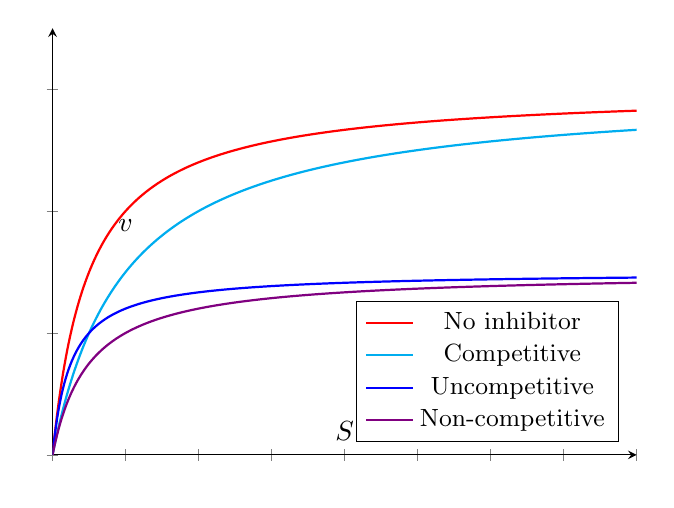
\begin{tikzpicture}
    \begin{axis}[
        width = 9cm,
        height = 7cm,
        legend pos = south east,
        x label style={at={(axis description cs:0.5,0.1)},anchor=north},
        y label style={at={(axis description cs:0.125,0.5)},rotate=270,anchor=south},
        xlabel = {$\con{S}$},
        ylabel = {$v$},
        axis lines = left,
        ymax = 3.5,
        domain = 0:8,
        samples = 400,
        xticklabels={},
        yticklabels={}
    ]
    \addplot [thick, red] {3/(1+0.5/x)};
    \addlegendentry{\small{No inhibitor}}
    \addplot [thick, cyan] {3/(1+1/x)};
    \addlegendentry{\small{Competitive}}
    \addplot [thick, blue] {3/(2+0.5/x)};
    \addlegendentry{\small{Uncompetitive}}
    \addplot [thick, violet] {3/(2+1/x)};
    \addlegendentry{\small{Non-competitive}}
    \end{axis}
\end{tikzpicture}
\end{document}
\end{figure}
\begin{figure}[H]
    \centering\documentclass{standalone}
\usepackage{PhysicalChemistryNote}
\begin{document}
\begin{tikzpicture}
    \begin{axis}[
        width = 9cm,
        height = 6cm,
        legend pos = north east,
        xlabel = {$\dfrac{1}{\con{S}}$},
        ylabel = {$\dfrac{1}{v}$},
        axis lines = center,
        ymax = 4,
        ymin = 0,
        domain = -6:10,
        samples = 400,
        xticklabels={},
        yticklabels={}
    ]
    \addplot [thick, red, domain=1:10] {0.5*x+1};
    \addlegendentry{\small{No inhibitor}}
    \addplot [thick, cyan, domain=1:10] {0.25*x+1};
    \addlegendentry{\small{Competitive}}
    \addplot [thick, blue, domain=1:10] {0.5*x+2};
    \addlegendentry{\small{Uncompetitive}}
    \addplot [thick, violet, domain=1:10] {x+2};
    \addlegendentry{\small{Non-competitive}}
    \addplot [thick, red, dashed, domain=-2:1] {0.5*x+1};
    \addplot [thick, cyan, dashed, domain=-4:1] {0.25*x+1};
    \addplot [thick, blue, dashed, domain=-4:1] {0.5*x+2};
    \addplot [thick, violet, dashed, domain=-2:1] {x+2};
    \end{axis}
\end{tikzpicture}
\end{document}
\end{figure}
\Part{多底物酶促反应——单置换反应与双置换反应}
\indent 实际情况中超过60\%的酶促反应都涉及两个及以上的底物.对双底物酶促反应的研究表明有以下几种机理.\\
\indent 如果两种底物\ce{A}和\ce{B}需要按照顺序与\ce{E}结合,然后生成产物,那么这样的机理被称为\tbf{单置换反应}.%
我们可以将机理表述如下.
\begin{tightcenter}
    \ce{E + A <=>T[$k_1$][$k_{-1}$] EA}\\
    \ce{EA + B <=>T[$k_2$][$k_{-2}$] EAB}\\
    \ce{EAB ->T[$k_3$] E + P + Q}
\end{tightcenter}
现在我们来推导单置换反应的速率方程.
\begin{derivation}\setcounter{equation}{0}
    仿照米氏方程的推导方式,对\ce{EA}和\ce{EAB}稳态近似可得
    \begin{equation}
        \dfrac{\di\con{EA}}{\di t}=k_1\con{E}\con{A}-k_{-1}\con{EA}-k_2\con{EA}\con{B}+k_{-2}\con{EAB}=0
    \end{equation}
    \begin{equation}
        \dfrac{\di\con{EAB}}{\di t}=k_2\con{EA}\con{B}-k_{-2}\con{EAB}-k_3\con{EAB}=0
    \end{equation}
    不妨令$K_{M,\ce{B}}=\dfrac{k_{-2}+k_3}{k_2}$为该反应对\ce{B}的米氏常数.由(2)可得
    \begin{equation}
        \con{EAB}=\dfrac{k_2\con{B}}{k_{-2}+k_3}\con{EA}=\dfrac{\con{B}}{K_{M,\ce{B}}}\con{EA}
    \end{equation}
    由(1)和(3)可得
    \begin{equation}
        \begin{aligned}
            \con{E}
            &= \dfrac{\left(k_{-1}+k_2\con{B}\right)\con{EA}-k_{-2}\con{EAB}}{k_1\con{A}} \\
            &= \dfrac{k_{-1}+k_2\con{B}-\dfrac{k_{-2}\con{B}}{K_{M,\ce{B}}}}{k_1\con{A}}\con{EA} \\
            &= \dfrac{k_{-1}+\dfrac{k_3}{K_{M,\ce{B}}}\con{B}}{k_1\con{A}}\con{EA}
        \end{aligned}
    \end{equation}
    这里由中间量$\con{EA}$统一变量可以降低计算的难度.\\
    这样,由(3)和(4),以及\ce{E}的物料守恒$\con{E}+\con{EA}+\con{EAB}=\con{E_0}$可得
    \begin{equation}
        \con{EA}
        =\dfrac{\con{E}}{\con{E}+\con{EA}+\con{EAB}}\con{E}_0
        =\dfrac{1}{\dfrac{k_{-1}+\dfrac{k_3}{K_{M,\ce{B}}}\con{B}}{k_1\con{A}}+1+\dfrac{\con{B}}{K_{M,\ce{B}}}}\con{E}_0
    \end{equation}
    于是反应的速率即为
    \begin{equation}
        \begin{aligned}
            v
            &= \dfrac{\di\con{P}}{\di t}=k_3\con{EAB}=\dfrac{k_2k_3\con{B}}{k_{-2}+k_3}\con{EA} \\
            &= \dfrac{1}{\dfrac{K_{M,\ce{B}}}{k_3\con{B}}}\cdot\dfrac{\con{E}_0}{\dfrac{k_{-1}+\dfrac{k_3}{K_{M,\ce{B}}}\con{B}}{k_1\con{A}}+1+\dfrac{\con{B}}{K_{M,\ce{B}}}} \\
            &= \dfrac{\con{E}_0}{\left(\dfrac{1}{k_3}+\dfrac{1}{k_1\con{A}}\right)+\dfrac{K_{M,\ce{B}}}{k_3}\left(1+\dfrac{k_{-1}}{k_1\con{A}}\right)\dfrac{1}{\con{B}}}
        \end{aligned}
    \end{equation}
    我们按照Lineweaver-Burk作图法的形式对(6)整理可得
    \begin{equation}
        \dfrac{1}{v}
        =\dfrac{1}{\con{E}_0}\left[\left(\dfrac{1}{k_3}+\dfrac{1}{k_1\con{A}}\right)+\dfrac{K_{M,\ce{B}}}{k_3}\left(1+\dfrac{k_{-1}}{k_1\con{A}}\right)\dfrac{1}{\con{B}}\right]
    \end{equation}
    以$\dfrac{1}{v}$对$\dfrac{1}{\con{B}}$作图,将得到斜率为$\dfrac{K_{M,\ce{B}}}{k_3\con{E}_0}\left(1+\dfrac{k_{-1}}{k_1\con{A}}\right)$,截距为$\dfrac{1}{\con{E}_0}\left(\dfrac{1}{k_3}+\dfrac{1}{k_1\con{A}}\right)$的直线.%
    因此,改变$\con{A}$,直线的斜率和截距将发生变化.这是单置换反应的特征.
\end{derivation}
如果底物\ce{A}与酶\ce{E1}反应后生成修饰形式的酶\ce{E2},然后与另一种底物\ce{B}反应生成原先的酶,如此循环往复,%
那么这样的机理被称为\tbf{双置换反应}.我们可以将机理表述如下.
\begin{tightcenter}
    \ce{E1 + A <=>T[$k_1$][$k_{-1}$] E1A ->T[$k_2$] E2 + P}\\
    \ce{E2 + B <=>T[$k_3$][$k_{-3}$] E2B ->T[$k_4$] E1 + Q}
\end{tightcenter}
现在我们来推导双置换反应的速率方程.
\begin{derivation}\setcounter{equation}{0}
    这一反应由两个相关的米氏反应构成.我们先对\ce{E1A}和\ce{E2B}稳态近似可得
    \begin{equation}
        \dfrac{\di\con{E1A}}{\di t}=k_1\con{E1}\con{A}-\left(k_{-1}+k_2\right)\con{E1A}=0\ \ \ \ \ \con{E1A}=\dfrac{\con{E1}\con{A}}{K_{M,\ce{A}}}
    \end{equation}
    \begin{equation}
        \dfrac{\di\con{E2B}}{\di t}=k_3\con{E2}\con{B}-\left(k_{-3}+k_4\right)\con{E2B}=0\ \ \ \ \ \con{E2B}=\dfrac{\con{E2}\con{B}}{K_{M,\ce{B}}}
    \end{equation}
    其中$K_{M,\ce{A}}$和$K_{M,\ce{B}}$分别为两步的米氏常数.\\
    体系处于稳态时,\ce{E1}和\ce{E2}的浓度也应当变化不大(否则就不满足\ce{E1A}和\ce{E2B}的稳态近似).于是有
    \begin{equation}
        \dfrac{\di\con{E1}}{\di t}=k_4\con{E_2B}+k_{-1}\con{E1A}-k_1\con{E1}\con{A}
    \end{equation}
    $(1)+(3)$可得
    \begin{equation}
        k_4\con{E2B}=k_2\con{E1A}
    \end{equation}
    结合(1)(2)和(4)和物料守恒$\con{E1}+\con{E1A}+\con{E2}+\con{E2B}=\con{E}_0$可得
    \begin{equation}
        \con{E1A}=\dfrac{\con{E}_0}{\dfrac{K_{M,\ce{A}}}{\con{A}}+1+\dfrac{k_2}{k_4}\left(\dfrac{K_{M,\ce{B}}}{\con{B}}+1\right)}
    \end{equation}
    于是反应的速率即为
    \begin{equation}
        v=k_2\con{E1A}=\dfrac{\con{E}_0}{\dfrac{1}{k_2}+\dfrac{1}{k_4}+\dfrac{K_{M,\ce{A}}}{k_2\con{A}}+\dfrac{K_{M,\ce{B}}}{k_4\con{B}}}
    \end{equation}
    我们按照Lineweaver-Burk作图法的形式对(6)整理可得
    \begin{equation}
        \dfrac{1}{v}=\dfrac{1}{\con{E}_0}\left[\dfrac{K_{M,\ce{B}}}{k_4}\dfrac{1}{\con{B}}+\left(\dfrac{1}{k_2}+\dfrac{1}{k_4}+\dfrac{K_{M,\ce{A}}}{k_2\con{A}}\right)\right]
    \end{equation}
    以$\dfrac1v$对$\dfrac{1}{\con{B}}$作图,将得到斜率为$\dfrac{K_{M,\ce{B}}}{k_4\con{E}_0}$,截距为$\dfrac{1}{\con{E}_0}\left(\dfrac{1}{k_2}+\dfrac{1}{k_4}+\dfrac{K_{M,\ce{A}}}{k_2\con{A}}\right)$的一条直线.%
    因此,改变$\con{A}$,直线的斜率不变而截距变化.这是双置换反应的特征.
\end{derivation}
\end{document}